\documentclass{article}
\usepackage{tikz}
\begin{document}
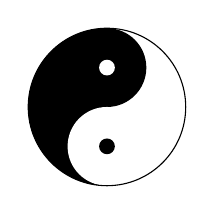
\begin{tikzpicture}
  %color one half of a unit circle
  \begin{scope}
    \clip (0,0) circle (1cm);
    \fill[black] (0cm,1cm) rectangle (-1cm, -1cm);
  \end{scope}
  %fill heads
  \fill[black] (0,0.5) circle (0.5cm);
  \fill[white] (0,-0.5) circle (0.5cm);
  %fill eyes
  \fill[white] (0,0.5) circle (0.1cm);
  \fill[black] (0,-0.5) circle (0.1cm);
  %outer line
  \draw (0,0) circle (1cm);
\end{tikzpicture}
\end{document}
